\newpage 
\chapter{ ساختار زمین ناقص و فراماده و تاثیر آنها بر کاهش تزویج}
\label{ch:3}
\section{مقدمه}
در این فصل با پیاده سازی ساختار ارائه شده در مقاله
\cite{carver1981microstrip}
و یک طرح فراماده مشهور تلاش بر کاهش کوپلینگ شده که در ادامه با توضیح هر کدام ساختار را برسی میکنیم.

\section{ساختار زمین ناقص}
ساختار زمین ناقص  با ایجاد نقص‌های مهندسی‌شده در صفحه زمین، توزیع جریان‌های سطحی را تغییر داده و باعث ایجاد خواص ممنوعه باندی
\LTRfootnote{Band-Stop}
 در پاسخ فرکانسی می‌شود. این ویژگی به‌طور مستقیم بر کاهش تزویج متقابل از طریق مهار انتشار امواج سطحی تأثیر می‌گذارد.
 
 
 ساختار DGS را می‌توان با یک مدار LC موازی مدلسازی کرد که در فرکانس رزونانس، امپدانس بالایی را ایجاد می‌کند و باعث مسدودسازی سیگنال می‌شود. مقادیر سلف ($L$) و خازن ($C$) به هندسه و ابعاد نقص ایجاد شده در صفحه زمین بستگی دارد.
 رابطه فرکانس رزونانس:
 \begin{align}
 	\label{eq:eq12}
	f_r = \frac{1}{2\pi\sqrt{LC}}
 \end{align}
 
 این مدل مدار معادل، درک بهتری از رفتار فرکانسی ساختار DGS و تأثیر آن بر کاهش کوپلینگ ارائه می‌دهد.
 
 
 \begin{figure}
	\centering
 	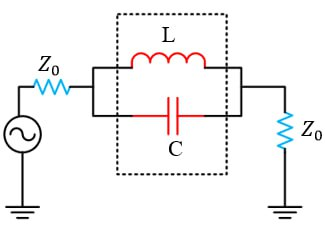
\includegraphics[scale=0.8]{Images/fig26.jpg}
 	\caption{معادل مداری ساختار زمین ناقص}
 	\label{fig26}
 \end{figure}
 
 در مقاله ی مد نظر ساختار انتخابی به صورت زیر میباشد: 
 
\begin{figure}
	\centering
	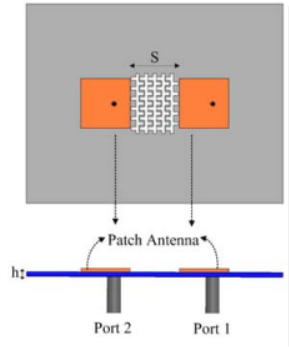
\includegraphics[scale=0.5]{Images/fig27.png}
	\caption{نمای بالایی و کناری از دو پچ آنتن به همراه DGS در صفحه ی زمین در آرایش E-Plain}
	\label{fig27}
 \end{figure}

\begin{figure}
	\centering
	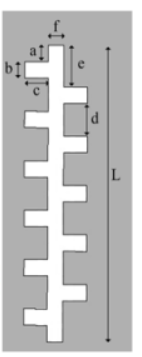
\includegraphics[scale=0.5]{Images/fig28.png}
	\caption{ارامتر های یک سلول DGS} % subcaption
	\label{fig28}
 \end{figure}
 
 
 با توجه به اینکه طراحی ارائه شده در مقاله مرجع
 \cite{carver1981microstrip}
 برای فرکانس کاری ۵ گیگاهرتز بهینه‌سازی شده است، جهت استفاده از این ساختار در فرکانس کاری مورد نظر این پروژه (۱.۴ گیگاهرتز)، لازم است ابعاد هندسی ساختار DGS به صورت متناسب اسکیل شوند. از آنجایی که ابعاد ساختارهای الکترومغناطیسی با طول موج رابطه مستقیم دارند، ضریب مقیاس ($\alpha$) از نسبت فرکانس‌ها محاسبه می‌شود: 
 
  \begin{align}
 	\label{eq:eq13}
 	\alpha = \frac{f_{\text{ref}}}{f_{\text{new}}} = \frac{5}{1.4} \approx 3.571
 \end{align}
 
 که در آن ۵ گیگ فرکانس کاری مقاله و 1.4 فرکانس جدید میباشد و در نتیجه ابعاد سلول DGS مقاله باید در 3.57 ضرب شوند.
 ابعاد قبل و بعد از محاسبه به صورت زیر میباشند : 
 \begin{center}
 \begin{tabular}{|c|c|c|}
 	\hline
 	74.55 & 21.0 & L \\
 	\hline
 	3.55 & 1.0 & a \\
 	\hline
 	3.55 & 1.0 & b \\
 	\hline
 	4.44 & 1.25 & c \\
 	\hline
 	8.17 & 2.3 & d \\
 	\hline
 	8.88 & 2.5 & e \\
 	\hline
 	3.55 & 1.0 & f \\
 	\hline
 \end{tabular}
 \end{center}
 
پس از اسکیل اولیه ابعاد بر اساس نسبت فرکانسی، شبیه‌سازی اولیه با پنج سلول DGS متوالی نتایج مطلوبی از نظر کاهش تزویج و تطبیق امپدانس در فرکانس هدف (۱.۴ گیگاهرتز) ارائه نداد. از این رو، بر اساس بررسی‌های تجربی، تغییرات زیر اعمال شد:
 \begin{enumerate}
 	\item{
 		تنظیم ابعاد سلول DGS:
 		
 		با توجه به مشاهدات، طول مؤثر هر سلول DGS می‌بایست تقریباً ۲۰ درصد بزرگتر از طول پچ  در نظر گرفته شود. با توجه به اینکه طول پچ محاسبه شده برای فرکانس ۱.۴ گیگاهرتز حدود ۷۵ میلیمتر بود، اما پس از ارزیابی‌های میدانی و بهینه‌سازی، طول بهینه سلول DGS ۱۴۰ میلی‌متر انتخاب شد. این تغییر باعث بهبود قابلیت مسدود سازی امواج سطحی در فرکانس هدف شد.
 		}
 	\item{
 	تغییر تعداد سلول‌ها:
 	
 	شبیه‌سازی‌ها نشان داد که استفاده از چهار سلول DGS (به جای پنج سلول) بهینه‌ترین نتایج را از نظر کاهش تزویج متقابل و حفظ عملکرد آنتن ارائه می‌دهد. افزایش تعداد سلول‌ها به پنج، نه تنها بهبود قابل توجهی در ایزولاسیون ایجاد نکرد، بلکه باعث افزایش تلفات و پیچیدگی غیرضروری شد.
 	}
 \end{enumerate}
 
 ساختار DGS بر روی آنتن پایه که در فصل قبل شبیه سازی کردیم در فاصله ی یک چهارم طول موج به صورت 
 \ref{fig29}
 و
 \ref{fig30}
  است.
  
 \begin{figure}
 	\centering
 	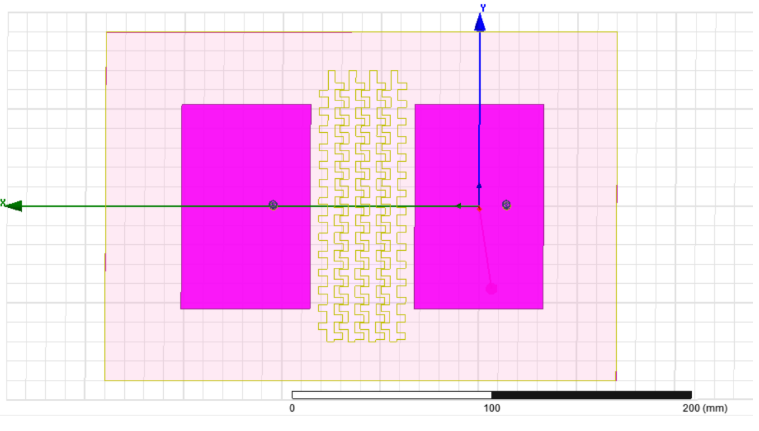
\includegraphics[scale=0.5]{Images/fig29.png}
 	\caption{نمای آنتن از پشت به همراه ۴ سلول DGS}
 	\label{fig29}
 \end{figure}
 
  \begin{figure}
 	\centering
 	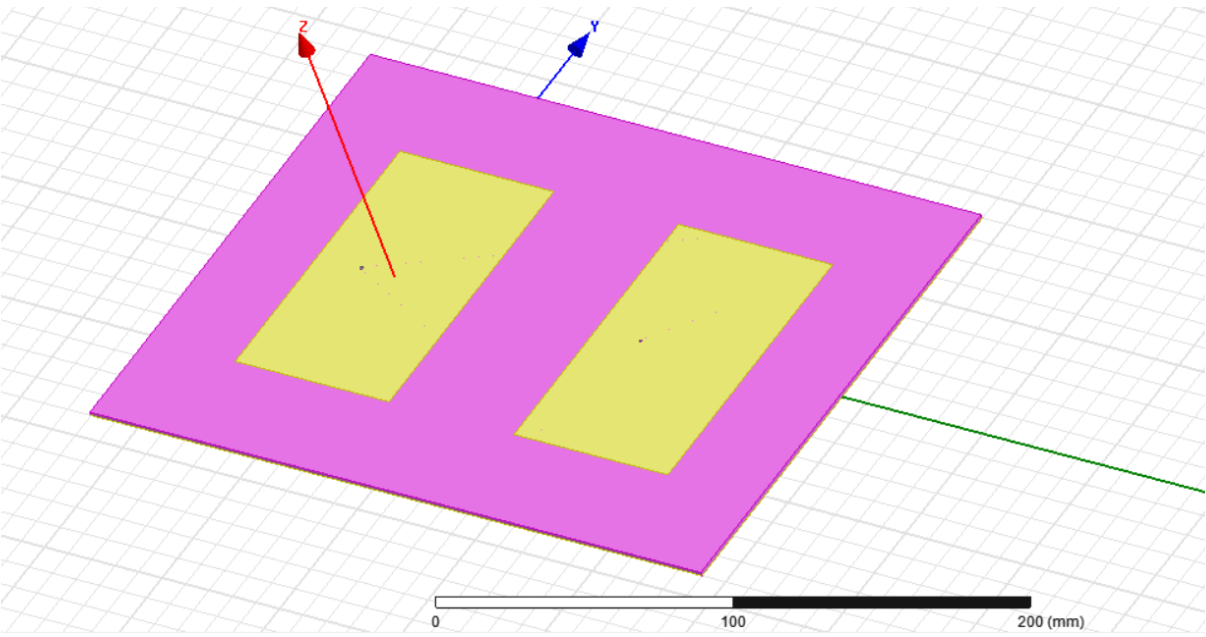
\includegraphics[scale=0.3]{Images/fig30.png}
 	\caption{نمای جلوی آنتن}
 	\label{fig30}
 \end{figure}
 
 
 \section{مقدار کاهش تزویج}
 
 پارامتر
 $S_{12}$
   (شاخص تزویج متقابل بین دو المان مجاور) در فرکانس کاری ۱.۴ گیگاهرتز، ۱۲ دسی‌بل کاهش یافت.
   
   
 این مقدار بهبود، کاملاً با نتایج گزارش‌شده در مقاله مرجع
 \cite{hajilou2012mutual}
 (که برای فرکانس ۵ گیگاهرتز طراحی شده بود) قابل مقایسه است و نشان‌دهنده کارایی روش اسکیل‌دهی و بهینه‌سازی اعمال‌شده است.
 
 \section{مقایسه با حالت پایه}
 در ساختار اولیه (فاقد DGS)، مقدار 
 $S_{12}$
 در حدود 
 $-22$
  دسی بل بود که پس از اعمال ساختار DGS بهینه‌شده، به 
  $-34$
    رسید. این بهبود ۱۲ دسی‌بلی، ایزولاسیون مطلوبی را برای کاربردهای عملی فراهم می‌کند.
\begin{figure}
	\centering
	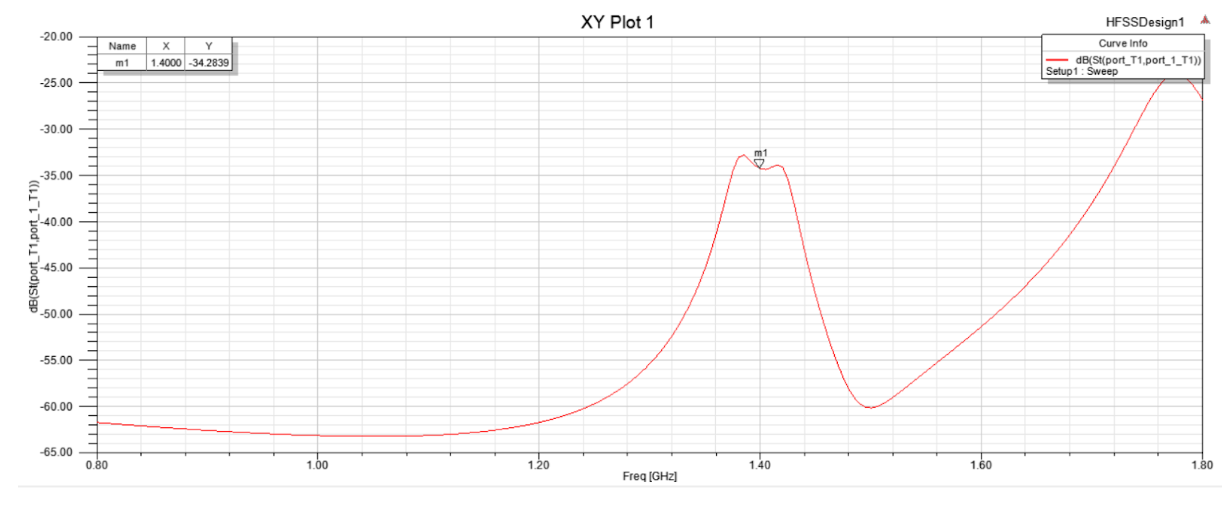
\includegraphics[scale=0.3]{Images/fig31.png}
	\caption{نمودار تزویج متقابل بین دو پورت آنتن}
	\label{fig31}
\end{figure}
    
\begin{figure}
	\centering
	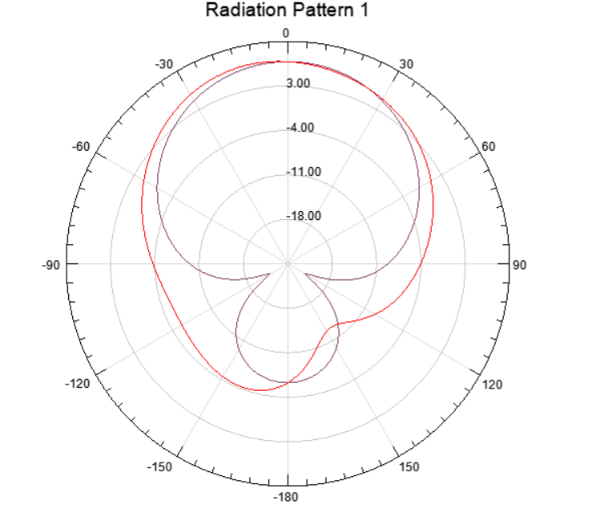
\includegraphics[scale=0.5]{Images/fig32.png}
	\caption{نمودار پترن تشعشعی}
	\label{fig32}
\end{figure}
 
 
\section{فراماده}
 فرامواد یا متامتریال
 \LTRfootnote{Metamaterial}
  ماده‌ای است که در طبیعت وجود ندارد و به صورت مهندسی شده آن را با استفاده از مواد موجود در طبیعت می‌سازند. به عنوان مثال با استفاده از ترکیب چند عنصر مانند فلزها و پلاستیک می‌توان شرایطی محیا کرد که خاصیت فراموادی داشته باشند. از ماده‌ی جدید ساخته شده می‌توان در کنترل موج‌های الکترومغناطیسی از طریق فیلتر کردن، جذب، افزایش یا حذف موج‌های ناخواسته استفاده کرد. یکی از ویژگی خاصی که فرامواد دارد، منفی بودن ضریب شکست است که توجه بسیاری از محققان را به خود جلب کرده است. 
  
  
  ابتدا این مواد به عنوان مواد چپ‌دستی (LH) مطرح شد تا برای همه اثبات شود که این مواد می‌توانند موج‌های الکترومغناطیسی را با استفاده از میدان الکتریکی، میدان مغناطیسی و بردارهای ثابت فاز با خاصیت‌ چپ‌دستی بودن در مقایسه با مواد موجود مرسوم که به عنوان مواد راست‌دستی (RH) شناخته شده‌اند، منتشر کند.
  
  
\subsection{ساختار فراماده}
 
 همانطور که می‌دانید ضریب شکست شامل دو پارامتر است، یکی ضریب گذردهی الکتریکی(
 $\varepsilon$)
  و دیگری ضریب نفوذ‌پذیری مغناطیسی(
  $\mu$).
   در سال ۲۰۰۰ ساختاری معرفی شد، ساختارهایی با 
   $\varepsilon$
   منفی/ 
   $\mu$
   مثبت با نام سیم نازک (TW) و
   $\varepsilon$
    مثبت/
    $\mu$
     منفی با نام رزوناتور حلقه‌ی شکافی (SRR) که در شکل 
     \ref{fig33}
      نشان داده شده است.
 \cite{seee}
 
  \begin{figure}
 	\centering
 	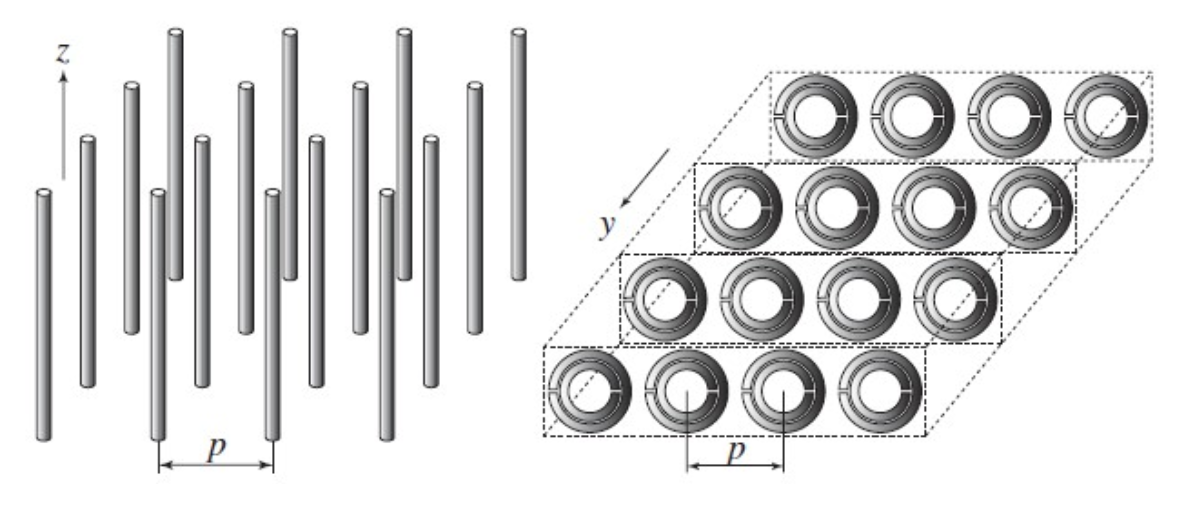
\includegraphics[scale=0.3]{Images/fig33.png}
 	\caption{ساختار های سیم نازک و حلقه رزوناتور شکافی}
 	\label{fig33}
 \end{figure}
 
 
 دانشمندان از این دو ساختار الهام گرفته و با ترکیب آنها توانستند اولین فرامواد چپ‌دستی را بصورت آزمایشگاهی تولید کنند. در شکل زیر ساختار پیشنهادی آنها نمایش داده شده است. یکی از مهم‌ترین ویژگی این نوع ساختار‌ها اندازه‌ی کوتاه‌تر از طول موج آنها است که موج‌های الکترومغناطیسی را تحت تاثیر خود قرار می‌دهد.
 
 
\begin{figure}
	\centering
	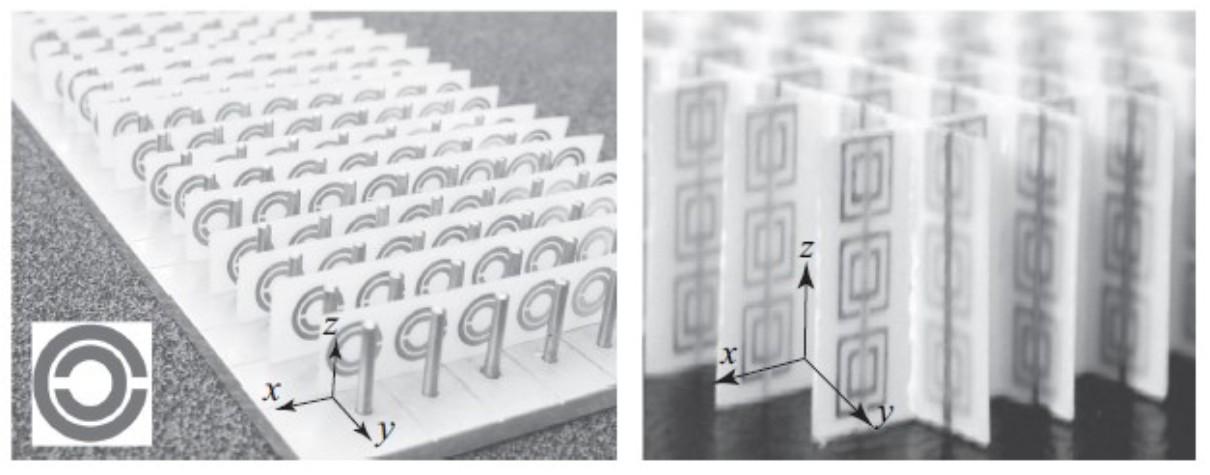
\includegraphics[scale=0.3]{Images/fig34.png}
	\caption{ساختار چپ دستی}
	\label{fig34}
\end{figure}

فراموادها در ساخت آنتن‌های با گین بالا کاربرد دارند. به طور پایه‌ای، سطوح فرامواد
\LTRfootnote{Metasurfaces}
 می‌توانند پلاریزاسیون میدان‌های الکترومغناطیسی را کنترل کنند.
این مواد به علت ساخت آسان و ظرفیت کنترل بالا بسیار مورد توجه است.

\subsection{کاربرد های فراسطح}
 کاربردهای فراسطح‌ها در آنتن‌های مایکرواستریپ:
\begin{enumerate}
	\item{
	بهبود بازده (گین): آنتن‌های صفحه‌ای گین کمی دارند که برای عملکرد مناسب باید این مشکل حل شود. برای این مهم می‌توان علاوه بر استفاده از آرایه‌ها، از فراسطح‌ها نیز کمک گرفت.
	}
	\item{
	کاهش ابعاد آنتن: اگر فراسطح‌ها را به عنوان صفحه زمین معیوب
	\LTRfootnote{Defective Ground Structure}
	 استفاده کنیم، می‌توانیم بدون کاهش کارایی، ابعاد آنتن را کاهش دهیم.
	}
	\item{
	بهبود پهنای باند فرکانسی: در این کاربرد، فراسطح را به عنوان بخشی از آنتن یا روی آنتن در نظر می‌گیریم.
	}
	\item{
	استفاده از فراسطح برای چندباندی کردن: گاهی می‌خواهیم چند باند فرکانسی برای کارهای مختلف در یک آنتن داشته باشیم که این باعث جذابیت ساختارهای چندباندی می‌شود. در این حالت هم می‌توان فراسطح را به عنوان عنصر تشعشعی یا قسمتی از صفحه زمین در نظر گرفت.
	}
	\item{
	کاهش تزویج متقابل : فراسطح‌ها با قابلیت کنترل امواج الکترومغناطیسی، می‌توانند به عنوان ساختارهای ایزوله‌کننده بین المان‌های آرایه آنتن عمل کنند. با ایجاد ممنوعیت باندی
	\LTRfootnote{Band-Stop}
	 در محدوده فرکانسی کاری، از انتقال انرژی ناخواسته بین المان‌ها جلوگیری کرده و تزویج متقابل را کاهش دهند. این ویژگی به ویژه در آرایه‌های فشرده (با فاصله کم بین المان‌ها) حیاتی است.
	}
\end{enumerate}

این ساختار به صورت آرایه ای رو یا بین آنتن قرار میگیرد(شکل
\ref{fig35}
و
\ref{fig36}
).

\begin{figure}
	\centering
	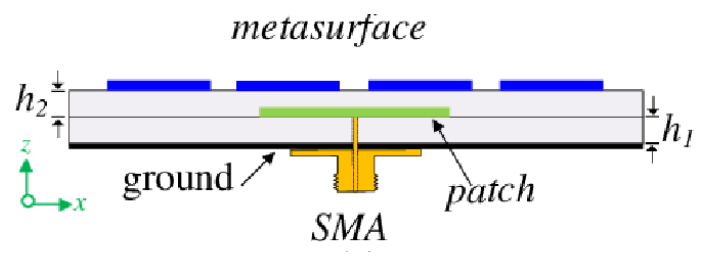
\includegraphics[scale=0.5]{Images/fig35.png}
	\caption{قرار فراماده روی یک پچ آنتن}
	\label{fig35}
\end{figure}

\begin{figure}
	\centering
	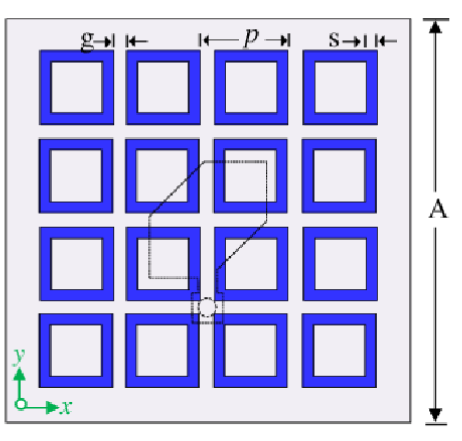
\includegraphics[scale=0.5]{Images/fig36.png}
	\caption{نمونه ای از آرایه ی فراماده}
	\label{fig36}
\end{figure}



\subsection{طراحی فراماده}
در این بخش از پروژه از سلول نشان داده شده در شکل
\ref{fig37}
 به عنوان المان فراماده استفاده میکنیم. در این ساختار از FR4 به عنوان زیر لایه و لایه ی رویی PEC میباشد.
\begin{figure}
	\centering
	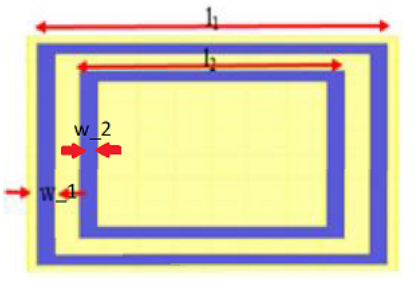
\includegraphics[scale=0.5]{Images/fig37.png}
	\caption{المان فراماده}
	\label{fig37}
\end{figure}

فرکانس تقریبی رزونانس این ساختار از فرمول 
\eqref{eq:eq14}
 بدست میآید

\begin{align}
	\label{eq:eq14}
	f_r \approx \frac{c}{2\pi\sqrt{\varepsilon_{e}} \cdot \frac{1}{\sqrt{L_{\text{eq}}C_{\text{eq}}}}}
\end{align}

که در آن
$L$
 معادل اندوکتانس حلقه و
 $ C $
 معادل خازن شکاف میباشد. البته از فرمول های زیر هم میتوان محدوده ی مثبت و منفی نفوذ پذیری و گذر دهی را محاسبه کرد.
\begin{align}
	\label{eq:eq15}
	\varepsilon_r \approx \frac{2}{jk_0d}\frac{1-\nu_1}{1+\nu_1}
\end{align}

\begin{align}
	\label{eq:eq15}
	\mu_r \approx \frac{2}{jk_0d}\frac{1-\nu_2}{1+\nu_2}
\end{align}

\begin{align}
	\label{eq:eq15}
	\nu_1=S_{21}+S_{11}
\end{align}


\begin{align}
	\label{eq:eq15}
	\nu_2=S_{21}-S_{11}
\end{align}
که
$ k_0$
 در اینجا عدد موج میباشد.
برای ابعاد حلقه های فراماده داریم:
 \begin{center}
	\begin{tabular}{|c|c|}
		\hline
		$I_1$ & 26.5 \\
		\hline
		$I_2$ & 15.9 \\
		\hline
		$W_1$ & 1.8 \\
		\hline
		$W_2$ & 2.6 \\
		\hline
	\end{tabular}
\end{center}

به دو شیوه فراماده را پیاده کردیم. شیوه اول دو آرایه بر روی لبه ی پچ در فاصله ی پنج میلیمتری از پچ که به صورت شکل
\ref{fig38}
و
\ref{fig39}
است.
\begin{figure}
	\centering
	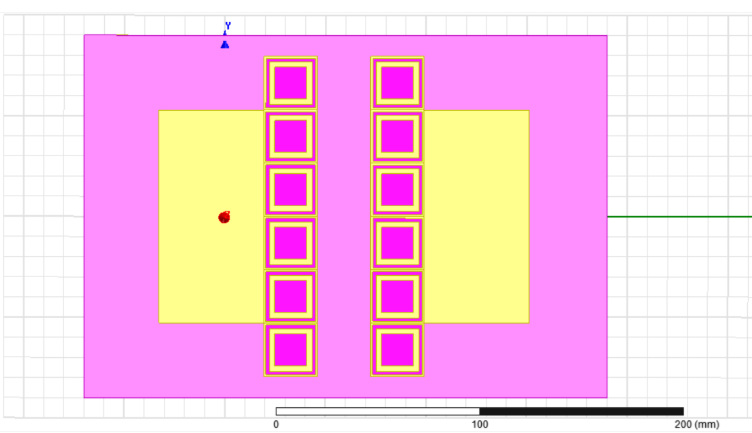
\includegraphics[scale=0.5]{Images/fig38.png}
	\caption{نمای بالای آنتن با آرایه فراماده}
	\label{fig38}
\end{figure}

\begin{figure}
	\centering
	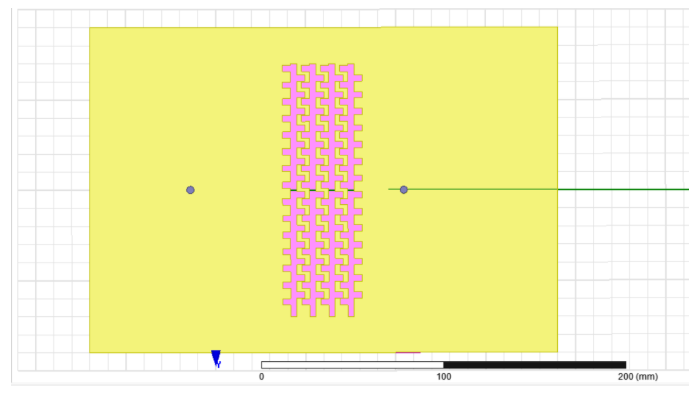
\includegraphics[scale=0.5]{Images/fig39.png}
	\caption{نمای پشت آنتن با DGS}
	\label{fig39}
\end{figure}

 نتیجه در شکل های 
\ref{fig40}
و
\ref{fig41}
نشان داده شده است.

\begin{figure}
	\centering
	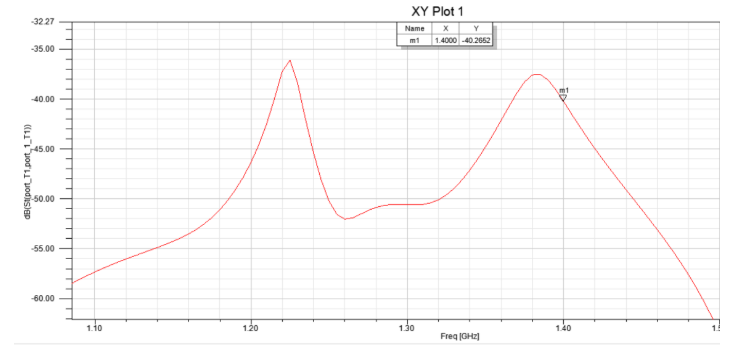
\includegraphics[scale=0.5]{Images/fig40.png}
	\caption{نمودار تزویج متقابل}
	\label{fig40}
\end{figure}


\begin{figure}
	\centering
	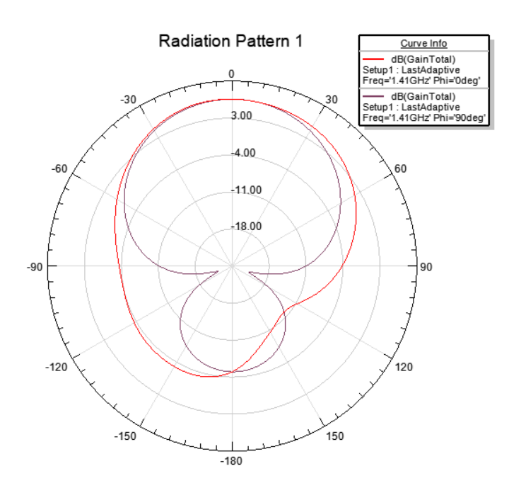
\includegraphics[scale=0.5]{Images/fig41.png}
	\caption{نمودار پترن تشعشعی}
	\label{fig41}
\end{figure}

همانطور که دیدیم مقدار کوپلینگ نسبت به حالت بدون فراماده حدود 6 دسی بل کاهش داشت. 
در شیوه ی دوم هر دو آرایه ی فراماده بین دو پچ مایکرواستریپ قرار دارند و نتایج شکل های
\ref{fig42}،
\ref{fig43}،
\ref{fig44}،
و
\ref{fig45}
نشان داده شده است.


\begin{figure}
	\centering
	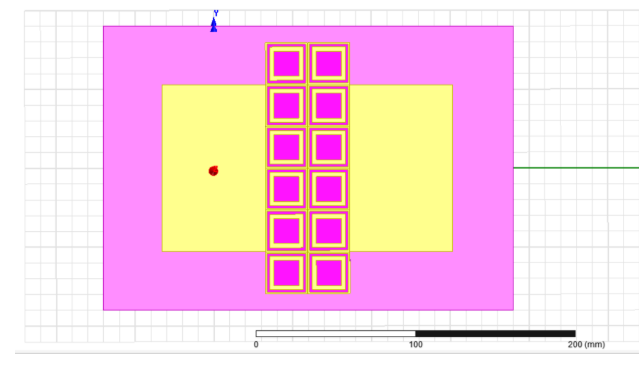
\includegraphics[scale=0.5]{Images/fig42.png}
	\caption{نمای بالای آنتن با فراماده}
	\label{fig42}
\end{figure}


\begin{figure}
	\centering
	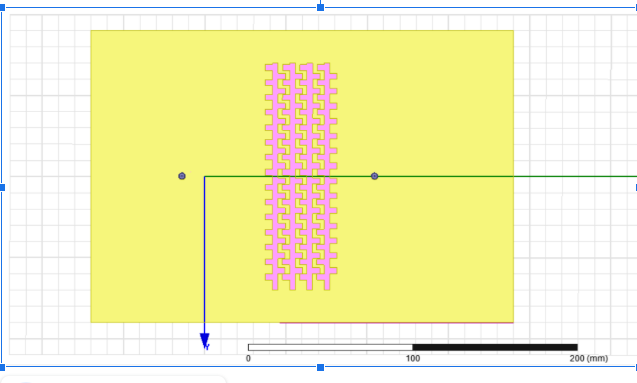
\includegraphics[scale=0.5]{Images/fig43.png}
	\caption{نمای پشت آنتن با DGS}
	\label{fig43}
\end{figure}

\begin{figure}
	\centering
	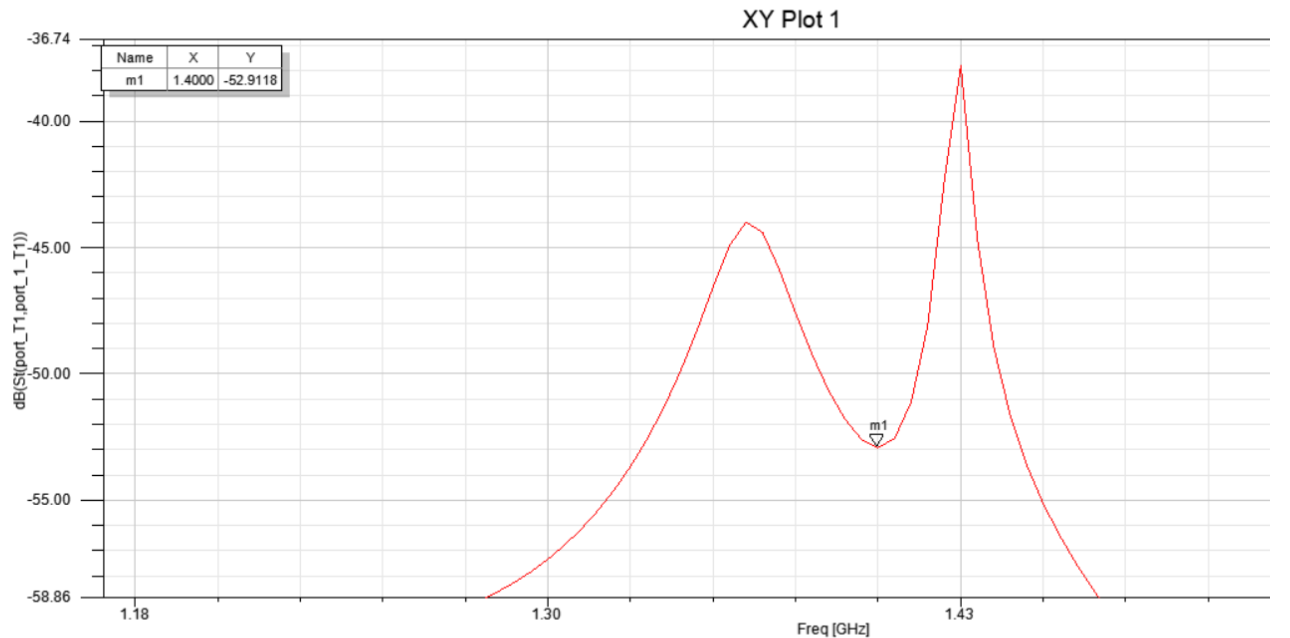
\includegraphics[scale=0.3]{Images/fig44.png}
	\caption{نمودار تزویج متقابل}
	\label{fig44}
\end{figure}

\begin{figure}
	\centering
	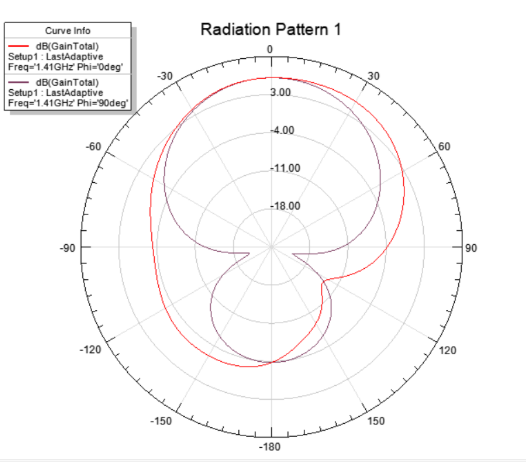
\includegraphics[scale=0.5]{Images/fig45.png}
	\caption{نمودار پترن تشعشعی}
	\label{fig45}
\end{figure}

\section{نتیجه گیری}
با توجه به مقادیر تزویج متقابل در روش های DGS و فرامادهبه ترتیب میتوان ۱۲ ، ۱۸ و ۳۲ دسی بل تزویج را کاهش داد. و این را به عنوان دو راه حل برای کاهش کوپلینگ در نظر گرفت.
